\documentclass{article}

\usepackage[margin=1in, top=1in, bottom=1.25in]{geometry}
\usepackage[utf8]{inputenc}
\usepackage[T1]{fontenc}
\usepackage{times}
\usepackage{microtype}
\usepackage{hyperref}
\usepackage{url}
\usepackage{booktabs}
\usepackage{amsmath}
\usepackage{amssymb}
\usepackage{graphicx}
\usepackage{caption}
\usepackage{subcaption}
\usepackage{xcolor}
\usepackage{natbib}
\usepackage{enumitem}
\usepackage{parskip}
\setlength{\parskip}{4pt}

\title{Perception Is How We Experience:\\
       Sensory Perceiver as a Typed Multimodal Architecture\\
       with Replay-Centric Continual Learning}

\author{
  Zach Shallbetter\\
  \textit{Independent Research}\\
  \texttt{zachshallbetter@icloud.com}
}

\begin{document}

\maketitle

\begin{abstract}
Sensory Perceiver is a multimodal architecture that combines modality-specific towers with shared cross-modal attention in settings where systems must keep learning over time. The implementation keeps modality identity explicit through runtime-validated MIME-style contracts, while the current empirical core is a replay-centric continual-learning program. On Split-CIFAR-100, feature-only replay fails with severe forgetting (CIL 4.86\%, BWT $-53.80\%$), raw-input replay with reservoir sampling materially improves retention (CIL 19.54\%, BWT $-34.91\%$), and the current tuned-core configuration improves the multiseed mean further to CIL 23.96\% and BWT $-30.39\%$ over six Titan runs. The strongest mechanistic conclusion is therefore that replay signals must reach shared feature extractors, not only late task heads.

The strongest completed perception-side evidence is the hardened synthetic sensor-routing ladder, where typed canonical routing outperforms merged routing on the baseline, capacity-matched control, leave-one-out branches, corruption branch, and two of three single-modality noise branches, with \texttt{noise\_robot\_arm} as the main exception. Real-data evidence is now reported conservatively with an explicit bootstrap-versus-canonical split: bootstrap runs on Speech Commands and WISDM are includable now, while bounded integrated sequences (\texttt{real-audio-seq-002} and \texttt{real-sensor-seq-001}) remain pending until their sequence reports complete successfully. The current contribution is therefore a disciplined blueprint for building domain-specific perception systems: keep modality identity explicit, validate routing semantics at the runtime boundary, and make continual-learning safeguards act on the shared perceptual backbone.
\end{abstract}

\section{Introduction}

Sensory Perceiver is motivated by a simple systems question: how should a perception model be structured if it must ingest heterogeneous sensory inputs, keep modality identity explicit, and continue adapting without full retraining each time new data arrives? The repository's answer combines three ideas:
\begin{enumerate}[leftmargin=*]
  \item modality-specific towers preserve sensor identity rather than collapsing heterogeneous streams into one generic input;
  \item a shared cross-modal core integrates those streams into a common latent representation;
  \item replay-centric continual learning attempts to preserve that shared representation over time.
\end{enumerate}

The broad framing is machine perception, but the evidence is intentionally bounded. The strongest validated result remains the continual-learning lane on Split-CIFAR-100. The strongest completed perception-side result is the synthetic sensor-routing ladder. Real-data support exists as bootstrap evidence on Speech Commands and WISDM, while the bounded integrated sequences remain pending. This manuscript follows that evidence boundary rather than the broadest architectural ambition.

\section{Related Work}

Sensory Perceiver sits at the intersection of multimodal integration, continual learning, and systems-oriented runtime design. The architectural lineage runs through attention-based sequence models and the Perceiver family, which demonstrated that a shared latent core can process heterogeneous inputs without a separate end-to-end architecture per modality. The continual-learning lineage runs through replay, reservoir sampling, EWC, SI, and gradient-projection methods, all of which address catastrophic forgetting from different directions.

The implementation here differs in emphasis. The central claim is not that MIME-style modality semantics are parsed directly inside model forward passes, but that explicit modality contracts at the runtime boundary reduce interface drift and make typed routing experimentally tractable. The empirical center of gravity is replay-path design: raw-input replay through the shared backbone matters much more in the current codebase than mild follow-on regularization.

\section{Methods}

\subsection{Architecture}

Each modality is routed through its own tower and then integrated through a shared cross-modal attention core. The current codebase treats modality identity as a canonical runtime concept rather than an implicit property of tensor shape. MIME-style modality registries are used for validation and setup derivation at the contract boundary, while downstream model dispatch remains modality-key based.

For live settings, the implementation now supports a stricter inference contract with structured per-modality payloads:
\begin{itemize}[leftmargin=*]
  \item \texttt{tensor}
  \item \texttt{valid\_mask}
  \item \texttt{status}
\end{itemize}
The preferred path is native mask-aware model support, with an explicit adapter available for legacy tensor-only models.

\subsection{Continual Learning}

The continual-learning program is replay-centric. Phase 1 used replay too high in the stack and failed badly. Phase 2 moved replay back to raw inputs with reservoir sampling, restoring replay gradients through shared feature extractors. The current tuned-core path improves on that configuration without changing the main conclusion: replay-path design is the strongest validated retention lever in this repository.

\subsection{Perception-Side Evaluation}

The completed synthetic perception-side ladder compares:
\begin{itemize}[leftmargin=*]
  \item \textbf{canonical}: typed modality routing with modality-specific towers,
  \item \textbf{merged}: one generic sensor stream without explicit typed modality separation.
\end{itemize}
It includes a baseline, a capacity-matched control, leave-one-out branches, binding corruption, and single-modality noise stress tests. Real-data evaluation now uses an explicit evidence taxonomy:
\begin{itemize}[leftmargin=*]
  \item \textbf{bootstrap}: first executable real-data runs used to validate ingestion and end-to-end operation,
  \item \textbf{canonical integrated}: bounded multi-dataset sequences promoted only after successful completion.
\end{itemize}

\section{Experiments}

\subsection{Continual-Learning Lane}

The continual-learning lane uses Split-CIFAR-100 as the narrow but code-aligned benchmark for catastrophic forgetting. The canonical current result is the tuned-core six-seed family executed on Titan Node. The associated figures and tables are generated directly from artifact-backed runs in the results package.

\subsection{Synthetic Sensor Routing Lane}

The synthetic sensor ladder is complete. It is the strongest completed perception-side evidence path, but it remains synthetic and therefore bounded. Its purpose is to test whether typed routing matters under controlled stress rather than to stand in for broad real-world multimodal validation.

\subsection{Real-Data Lane}

The real-data lane is intentionally conservative. Bootstrap evidence is includable now:
\begin{itemize}[leftmargin=*]
  \item \texttt{real-audio-seq-001} on \texttt{speech\_commands}
  \item \texttt{real-seq-004} on \texttt{wisdm}
\end{itemize}
Canonical integrated evidence is still pending:
\begin{itemize}[leftmargin=*]
  \item \texttt{real-audio-seq-002} on \texttt{speech\_commands}, \texttt{esc50}, \texttt{urbansound8k}, and \texttt{fsd50k}
  \item \texttt{real-sensor-seq-001} on the integrated real-sensor lineup including \texttt{realworld\_har}
\end{itemize}
Deferred legacy sources remain explicit but are no longer part of the active bounded chain:
\begin{itemize}[leftmargin=*]
  \item \texttt{audioset}: replaced operationally by \texttt{fsd50k}
  \item \texttt{ubiqlog}: replaced operationally by \texttt{realworld\_har}
\end{itemize}

\section{Results}

\subsection{Continual-Learning Core}

The current artifact-backed continual-learning story is summarized by the generated results package:
% Auto-generated by paper/figures/build_results_package.py
% Drop-in snippet for the Split-CIFAR-100 results section.

\begin{table}[t]
  \centering
  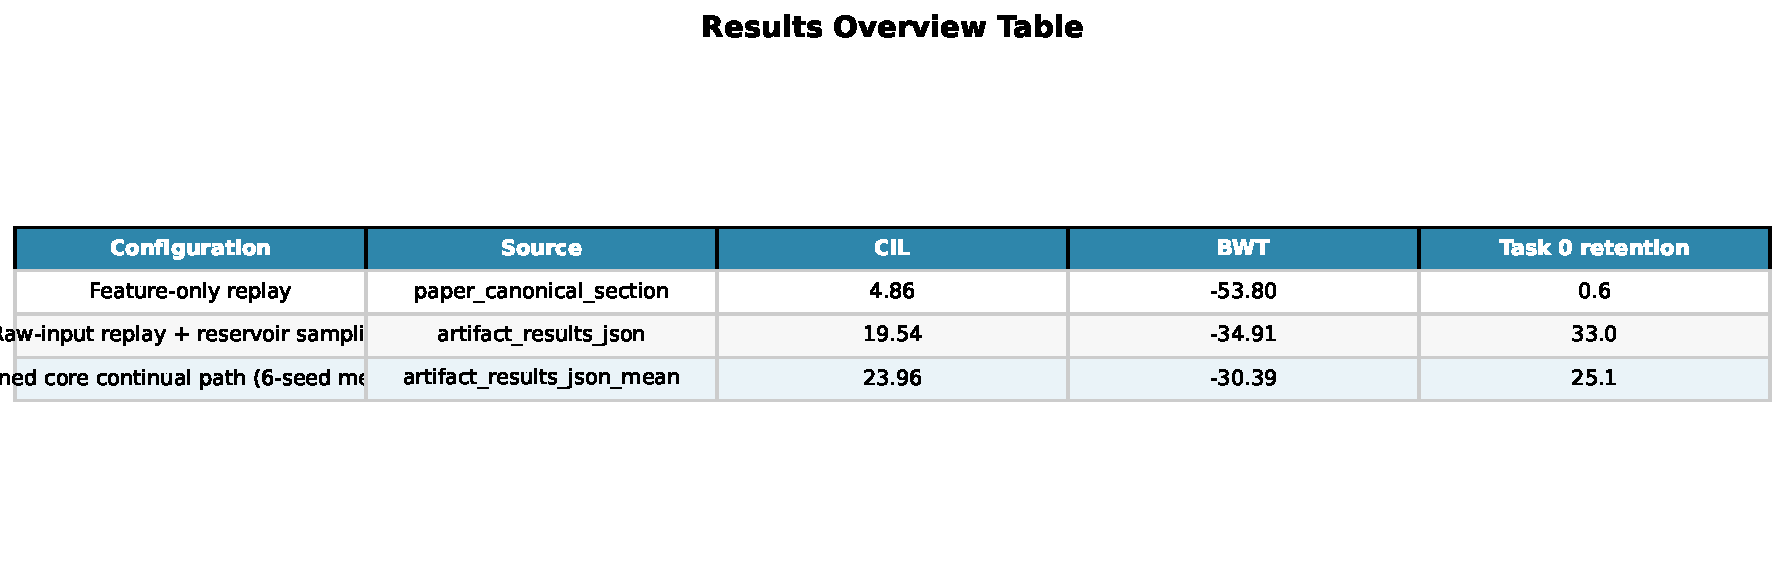
\includegraphics[width=\linewidth]{../figures/generated/results_package/table_results_overview.pdf}
  \caption{Split-CIFAR-100 continual-learning progression. Phase 1 is a legacy feature-only replay result sourced from the canonical paper section because the original run directory is not currently tracked as a local artifact. Phase 2 and Phase 3 are artifact-backed, with Phase 3 reporting the mean over 6 tuned-core Titan runs from family `20260311_140818`.}
  \label{tab:split-cifar-results-overview}
\end{table}

\begin{figure}[t]
  \centering
  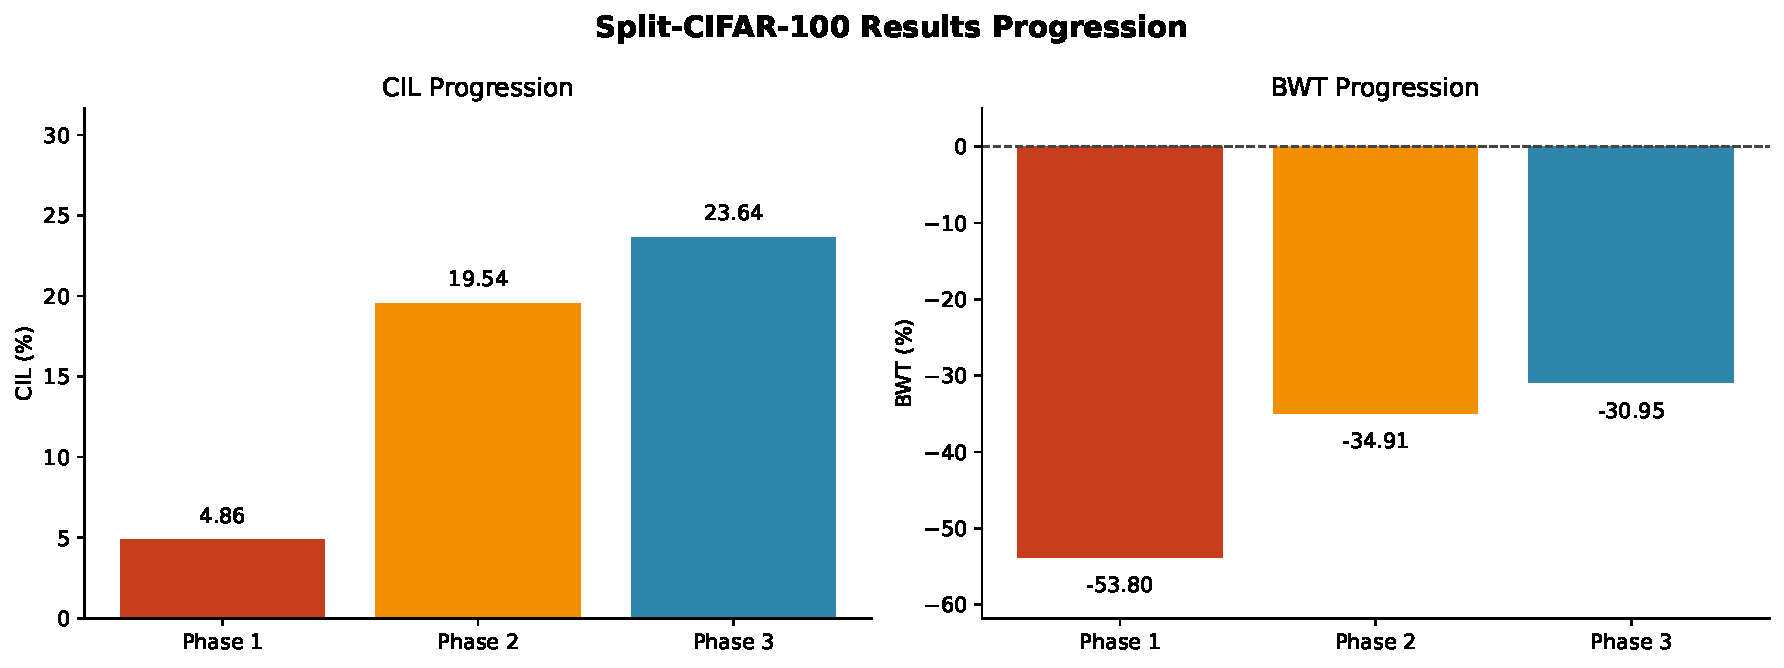
\includegraphics[width=\linewidth]{../figures/generated/results_package/figure_phase_progression.pdf}
  \caption{CIL and BWT progression from feature-only replay to raw-input replay with reservoir sampling and then the tuned-core continual configuration. The figure emphasizes that replay-path design, not just stronger regularization, drove the major retention gains.}
  \label{fig:split-cifar-phase-progression}
\end{figure}

\begin{figure}[t]
  \centering
  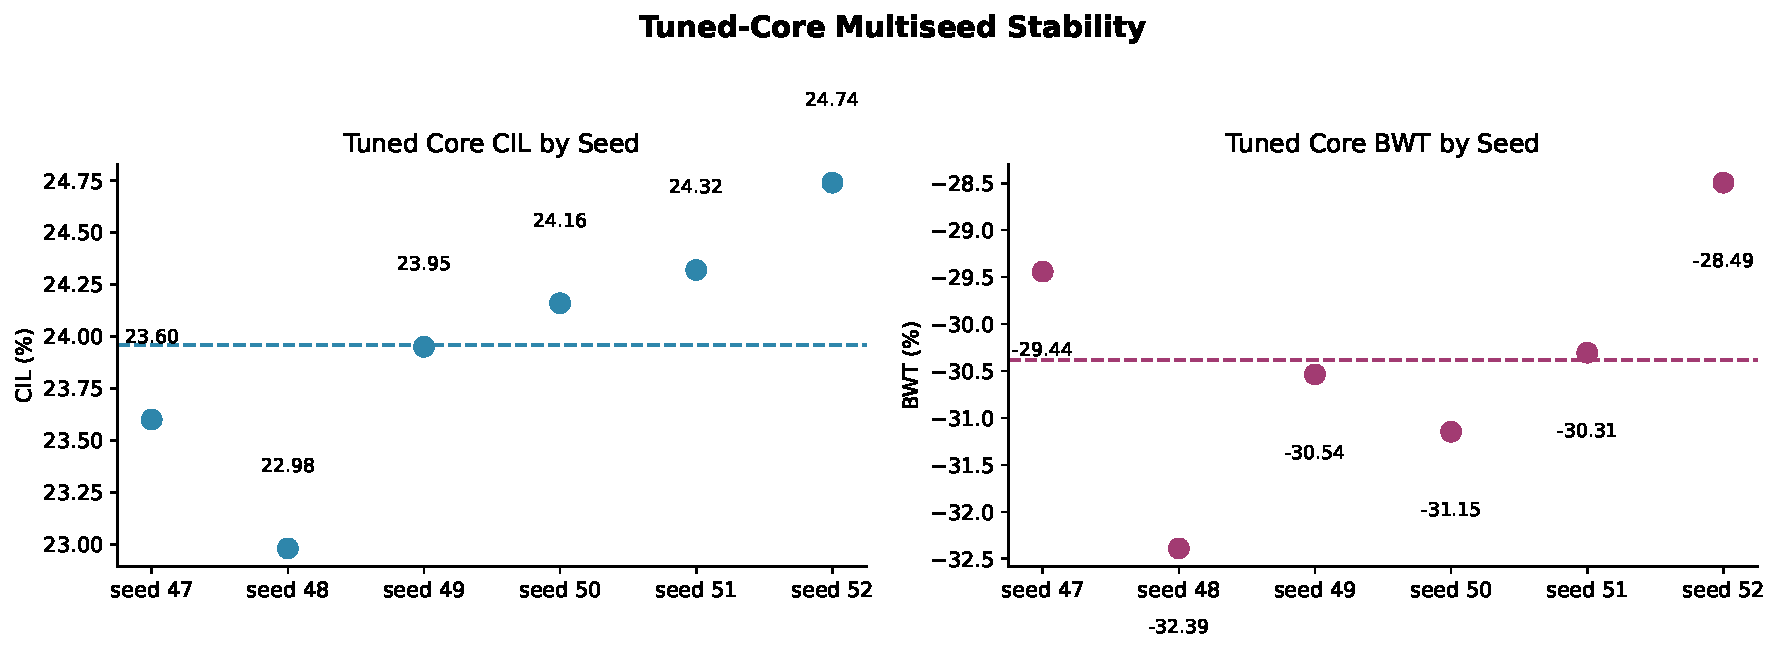
\includegraphics[width=\linewidth]{../figures/generated/results_package/figure_tuned_core_multiseed.pdf}
  \caption{Tuned-core multiseed stability on Titan Node. Each point is one full 20-task Split-CIFAR-100 run, with dashed lines indicating the multiseed means. Variance is modest relative to the mean effect size.}
  \label{fig:tuned-core-multiseed}
\end{figure}

\begin{figure}[t]
  \centering
  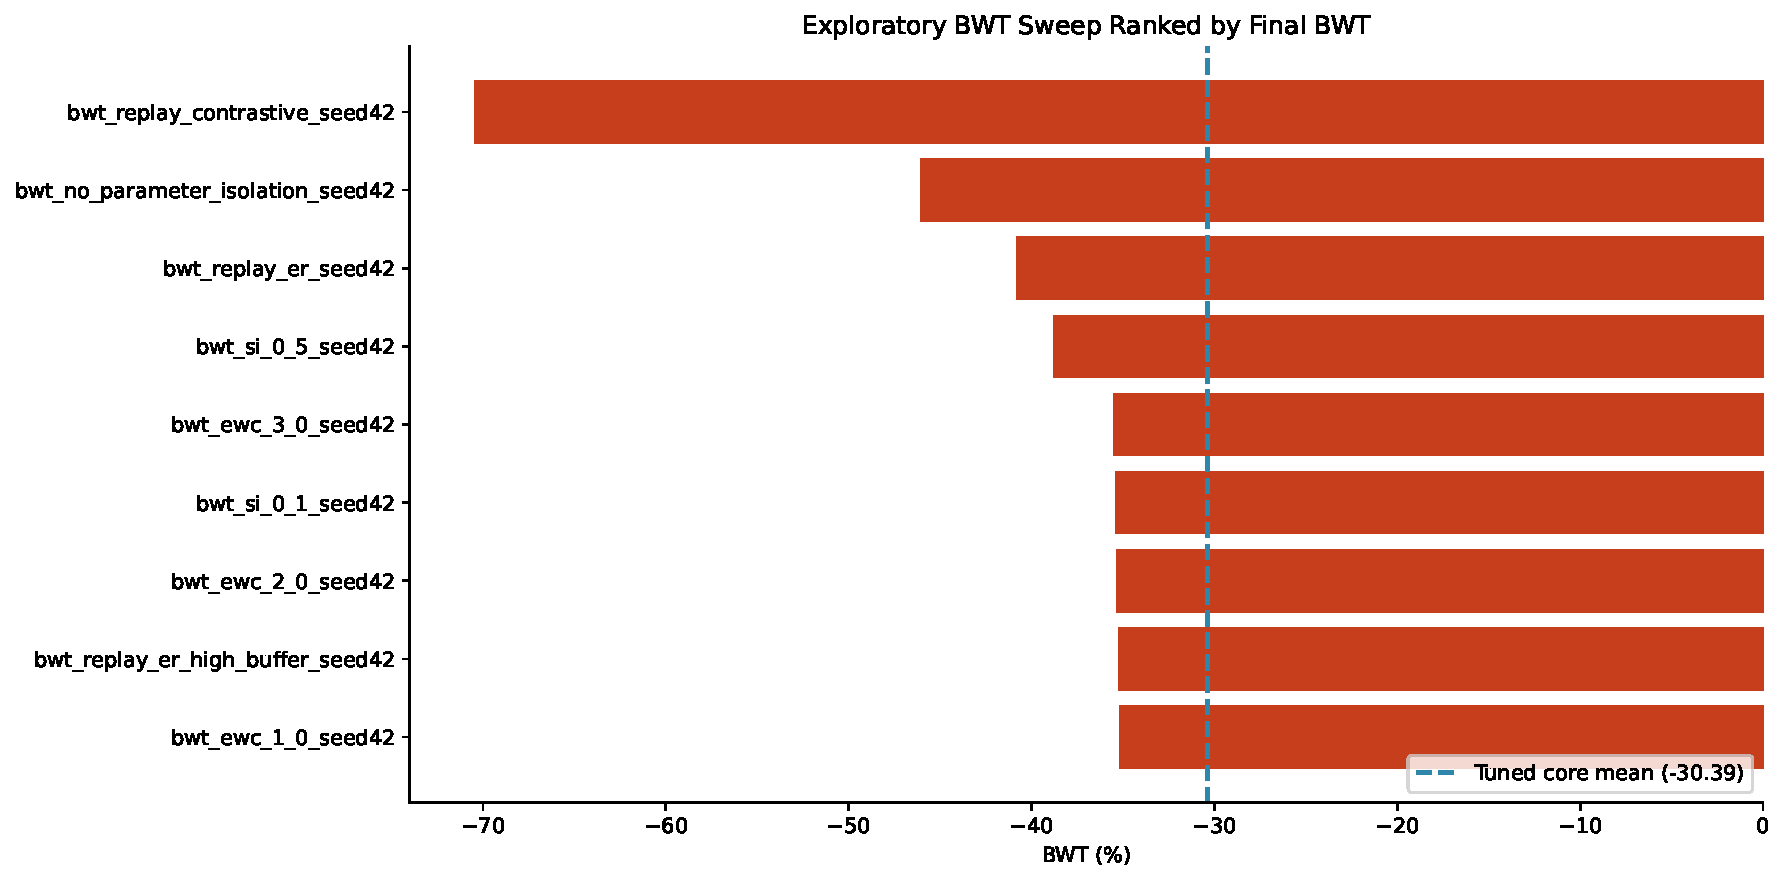
\includegraphics[width=\linewidth]{../figures/generated/results_package/figure_bwt_sweep_ranked.pdf}
  \caption{Exploratory BWT sweep ranked by final BWT. The dashed reference line marks the tuned-core multiseed mean. None of the completed EWC, SI, larger-buffer ER, or contrastive replay runs surpass the tuned-core baseline.}
  \label{fig:bwt-sweep-ranked}
\end{figure}

\begin{figure}[t]
  \centering
  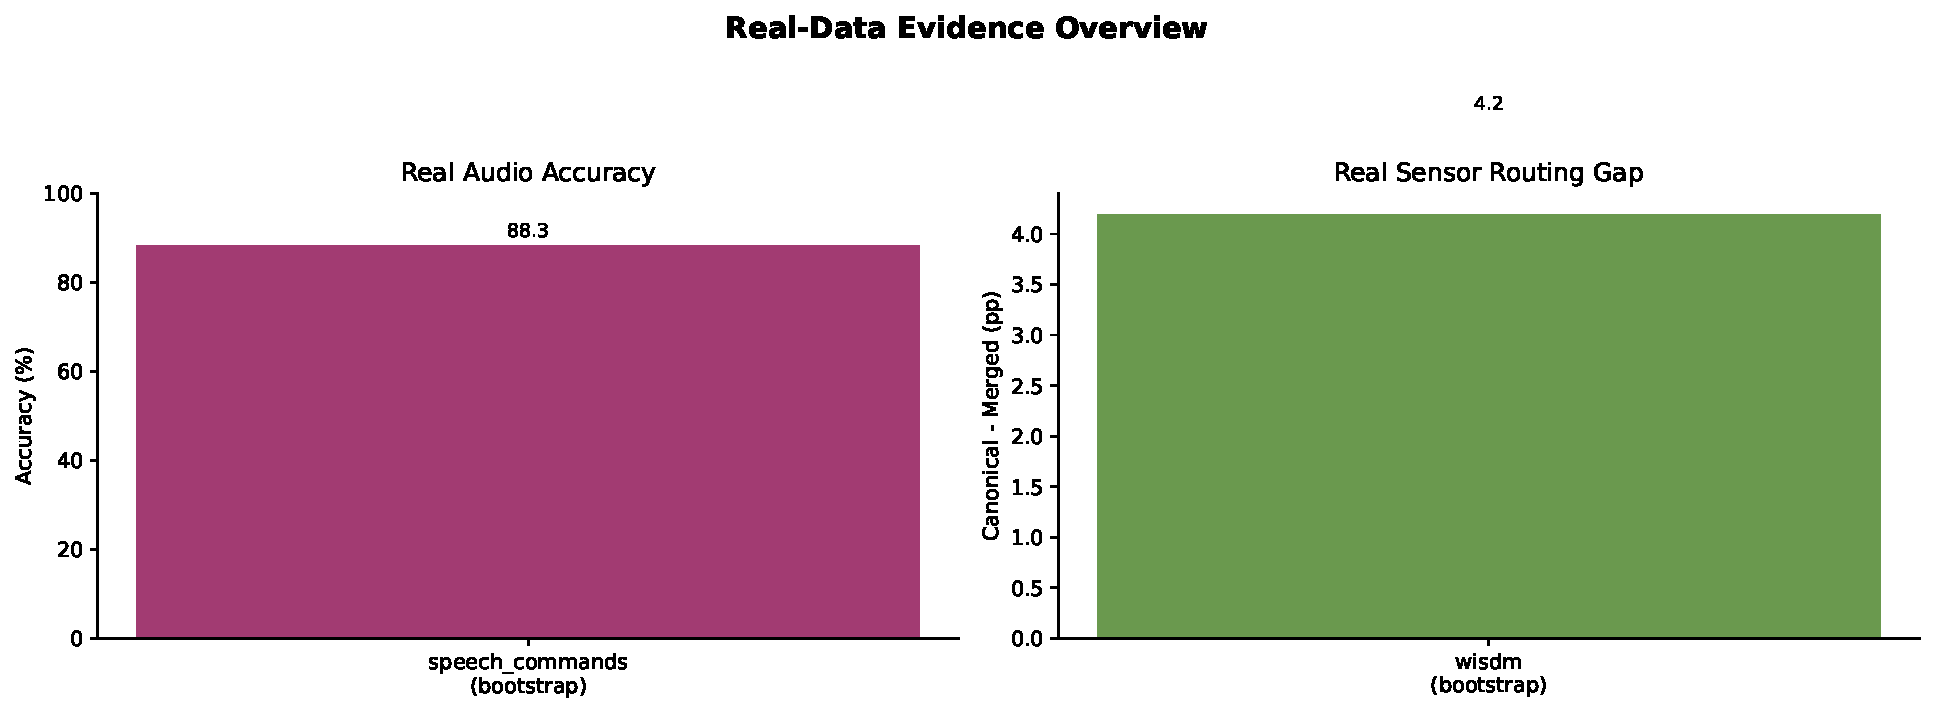
\includegraphics[width=\linewidth]{../figures/generated/results_package/figure_real_data_evidence.pdf}
  \caption{Real-data evidence overview. Bootstrap evidence comes from `real-audio-seq-001` on Speech Commands and `real-seq-004` on WISDM. Canonical evidence is promoted from `real-audio-seq-002` and `real-sensor-seq-001` as those bounded integrated sequences complete. Historical bootstrap reports may still list newly integrated datasets as candidates, so the package treats sequence stage and current supervisor defaults as the canonical source of truth.}
  \label{fig:real-data-evidence-overview}
\end{figure}


The tuned-core six-seed result is the strongest validated configuration in the codebase:
\begin{itemize}[leftmargin=*]
  \item CIL mean: 23.96\%
  \item BWT mean: $-30.39\%$
  \item Task 0 retention mean: 25.1\%
\end{itemize}
The exploratory BWT sweep remains useful negative evidence: none of the completed EWC, SI, larger-buffer ER, or contrastive replay settings surpass the tuned-core baseline.

\subsection{Completed Synthetic Sensor Routing Evidence}

The completed synthetic sensor ladder establishes the strongest finished perception-side result in the repository. Canonical typed routing is ahead on the baseline, the capacity-matched control, all leave-one-out branches, the binding-corruption branch, and two of the three single-modality noise branches. The paired gaps are:
\begin{itemize}[leftmargin=*]
  \item baseline: $+0.4583$
  \item capacity-matched baseline: $+0.3767$
  \item drop smartwatch: $+0.3317$
  \item drop room environment: $+0.7950$
  \item drop robot arm: $+0.6333$
  \item corrupt bindings: $+0.2717$
  \item noise smartwatch: $+0.0633$
  \item noise room environment: $+0.0617$
  \item noise robot arm: $-0.0933$
\end{itemize}
The supervisor's final state for the ladder is \texttt{canonical-dominant}. The important nuance is that the result is strong but not uniform: \texttt{noise\_robot\_arm} is the one completed branch where merged routing wins.

\subsection{Bootstrap Real-Data Evidence}

Figure~\ref{fig:real-data-evidence-overview} summarizes the current real-data package state. The completed bootstrap results are:
\begin{itemize}[leftmargin=*]
  \item \texttt{real-audio-seq-001} on Speech Commands: mean accuracy 88.32\%
  \item \texttt{real-seq-004} on WISDM: canonical-minus-merged gap $+4.19$ percentage points
\end{itemize}
These runs establish that the first real audio and real sensor paths work end to end on Titan, but they are not yet the canonical integrated comparison set for the next paper update. The generated package under \texttt{paper/figures/generated/results\_package/real\_data/} is the source of truth for bootstrap-versus-canonical status.

\section{Discussion}

\subsection{What Is Strongest Right Now}

The strongest evidence in the repository is still replay-centric continual learning. The central mechanistic insight survives every implementation pass so far: replay must reach shared feature extractors, not only late task heads. The tuned-core Split-CIFAR-100 result is therefore still the main quantitative anchor for the paper.

\subsection{What The Synthetic Sensor Ladder Adds}

The completed synthetic sensor ladder materially strengthens the broader perception story. It shows that typed routing is not just runtime hygiene; it changes performance on a controlled benchmark, survives a capacity-matched control, and remains favorable under multiple structured stressors. At the same time, the \texttt{noise\_robot\_arm} reversal prevents overclaiming. The right interpretation is ``strong controlled support'' rather than ``uniform dominance.''

\subsection{What The Real-Data Lane Adds}

The real-data lane now matters because it prevents the project from staying trapped in synthetic-only evidence. Bootstrap Speech Commands and WISDM runs prove that the real-data path is executable. However, the paper should still treat the integrated sequences as pending. This bootstrap-versus-canonical split is the main guardrail against overstating progress while Titan is still running bounded evidence chains.

\subsection{Claim Surface Versus Evidence Surface}

The architectural concept is broader than the current evidence. That is acceptable only if the manuscript stays explicit about the gap. Today the evidence hierarchy is:
\begin{enumerate}[leftmargin=*]
  \item strongest validated result: replay-centric continual learning,
  \item strongest completed perception-side result: synthetic sensor routing ladder,
  \item completed bootstrap real-data evidence: Speech Commands and WISDM,
  \item canonical integrated real-data evidence: pending.
\end{enumerate}
That hierarchy is the one this manuscript defends.

\subsection{Practical Interpretation}

For an applied reader, the present result is not a finished universal perception product. It is a disciplined blueprint for building domain-specific systems that:
\begin{itemize}[leftmargin=*]
  \item keep modality identity explicit,
  \item validate modality semantics at the runtime boundary,
  \item remain useful when one stream is degraded,
  \item and adapt over time without constant full retraining.
\end{itemize}

\section{Conclusion}

Sensory Perceiver now has one coherent evidence story. Replay-centric continual learning remains the strongest validated result, with the tuned-core six-seed Titan family as the current quantitative anchor. The completed synthetic sensor ladder provides the strongest finished perception-side evidence, showing a strong but not unconditional advantage for typed routing. Bootstrap real-data evidence on Speech Commands and WISDM establishes that the real-data path is executable, while canonical integrated sequences remain explicitly pending until their bounded reports complete successfully.

This is the right stopping point for the current manuscript. It does not overclaim in-flight runs, it preserves blocked states such as AudioSet media acquisition and UbiqLog task definition, and it keeps the broad machine-perception framing tied to what the code and artifacts actually support. If the pending integrated sequences complete successfully, the next revision can promote them into the canonical results package. Until then, the present paper should be read as a code-aligned architecture paper with a strong continual-learning core, a completed synthetic perception-side ladder, and a cautiously advancing real-data evidence path.

\bibliographystyle{abbrvnat}
\bibliography{references}

\end{document}
